\chapter{Evaluation}\label{chapter:Evaluation}


\section{Accessibility Results}
In order to provide a comprehensive analysis of the amount and type of accessibility violations, 
we divide the analysis into 3 categories. We report both a quantitive with aggregate 
metrics and a qualitive analysis with fine-grained explanations.

\subsection{Quantitive Analysis}
\subsubsection{Prompting Techniques}
Figure xy illustrates the comparison of the average amount of violations, the
Inaccessibility Rate (IR) and the Impact-Weighted Inaccessibility Rate (IWIR) between 
the human baseline and the models with the corresponding prompting techniques.

\paragraph{Key observations:}
Even the weakest LLM outperforms the human baseline regarding the average amount
of violations per webpage and the IR. Only the IWIR remains constant, only showing small 
differences across the models. The human-written HTML/CSS of our dataset counts 1339 accessibility 
violations, leading to $\sim$25.26 violations per file across the whole dataset.
On the other hand, even gemini with the naive prompting technique,
the worst performing set of parameter, had a maximum of 917 accessibility 
violations, leading to $\sim$17.3 violations per file across the whole dataset.\newline
GPT‑4o achieved the lowest average amount of violations per webpage, IR and IWIR.\newline
Advanced prompting techniques show only little effect, compared to the naive baseline, 
demonstrating the LLMs' inherent understanding of accessibility. 
Even if the naive prompting approach does not instruct the LLMs to generate
code with compliance to the WCAG standards, it still only shows slightly 
increased amounts of violations than more advanced prompting techniques.



\paragraph{Error Distribution:}
Figure yxc illustrates the distribution of violations per WCAG success criterion.
The distribution shows a similar left-skewed distribution across all models, indicating 
that the models have a similar understanding of the WCAG rules.\newline
At least 65\% of all violations are caused by color contrast and 
landmark and region issues. This finding is not only consistent across the different models
and prompting techniques, but also in human-written code.
\newline
The following types of violations are mainly caused by missing labels, wrong link colors, 
issues with header tags and the size of frontend components. This demonstates that only 
a small subset of WCAG violations have relevant and non-negligible amount of violations. 
Especially GPT-4o shows illustrates this clearly, as only 6 types of violations cause 
94\%(number check) of all violations.\newline
The results also show differences between the models. While gemini seems to have more color 
contrast violations, landmark and region rules cause
more problems for the GPT-4o model.


\begin{table}[htbp]
  \centering
  \footnotesize
  \caption{Accessibility benchmarks: Inaccessibility Rate (IR), Impact‑Weighted
           Inaccessibility Rate (IWIR), Average Number of Violations per webpage
           (ANV) and Total Violations (TV).}
  \label{tab:webcode2m}
  \setlength{\tabcolsep}{4pt}
  \begin{tabular}{l *{3}{cccc}} 
    \toprule
    \multirow{2}{*}{\textbf{Technique}} &
      \multicolumn{4}{c}{\textbf{Gemini Flash 2.0}} &
      \multicolumn{4}{c}{\textbf{ChatGPT‑4o}} &
      \multicolumn{4}{c}{\textbf{Qwen2.5vl‑7B}} \\

    \cmidrule(lr){2-5}\cmidrule(lr){6-9}\cmidrule(l){10-13}
      & IR & IWIR & ANV & TV
      & IR & IWIR & ANV & TV
      & IR & IWIR & ANV & TV \\
    \midrule
    Naive                & 0.1142 & 0.4770 & 15.45 & 819 & 0.1222 & 0.4710 & 13.75 & 729 & 0.1070 & 0.4025 & 6.21 & 329 \\
    Zero‑Shot            & 0.1033 & 0.4774 & 14.25 & 755  & 0.1002 & 0.4735 & 12.33 & 653  & 0.1094 & 0.3906 & 5.53 & 293 \\
    Few‑Shot             & 0.1093 & 0.4791 & 15.74 & 834  & 0.0796 & 0.4464 & 9.49 & 503  & 0.0823 & 0.4092 & 5.92 & 314 \\
    CoT            & 0.1107 & 0.4831 & 14.28 & 757  & 0.0861 & 0.4453 & 10.04 & 532 & \underline{\textbf{0.0689}} & 0.4599 & 6.49 & 344 \\
    IterativeRef1     & 0.0308 & 0.3872 & 5.85 & 310  & 0.0173 & 0.3188 & 2.43 & 129  & 0.0956 & 0.3513 & 5.79 & 307 \\
    IterativeRef2     & 0.0175 & 0.2596 & 3.45 & 183  & 0.0076 & 0.2128 & 1.09 & 58  & 0.0830 & 0.2875 & 5.17 & 274 \\
    IterativeRef3     & \underline{\textbf{0.0136}} & \underline{\textbf{0.2148}} & 2.77 & 147
                         & \underline{\textbf{0.0044}} & \underline{\textbf{0.1356}} & \underline{\textbf{0.68}} & \underline{\textbf{36}}
                         & 0.0768 & \underline{\textbf{0.2775}} & 5.04 & 267 \\
    Composite            & 0.0174 & 0.3493 & \underline{\textbf{2.58}} & \underline{\textbf{137}} & 0.0235 & 0.3368 & 3.34 & 177  & 0.0898 & 0.4044 & \underline{\textbf{4.96}} & \underline{\textbf{263}} \\
    Agent                & 0.0836 & 0.4700 & 13.08 & 693  & 0.0886 & 0.4180 & 11.28 & 598  & 0.0997 & 0.4042 & 6.08 & 322 \\
    \bottomrule
\addlinespace[2pt]
\textbf{Human Baseline} & \textbf{0.1131} & \textbf{0.565} & \textbf{25.26} & \textbf{1339} 
                        & \textbf{0.1131} & \textbf{0.565} & \textbf{25.26} & \textbf{1339} 
                        & \textbf{0.1131} & \textbf{0.565} & \textbf{25.26} & \textbf{1339} \\
\bottomrule
  \end{tabular}
\end{table}





\subsection{Qualitive Analysis}
\subsubsection{Consistency}
We model the consistency of violations found within different 
experiment runs and dataset entries. Therefore, we use the \textit{cosine-similarity} for 
each k-dimenstional error vector, where each dimension represents the amount of a specific 
WCAG violation. The cosine-similarity is then calculated between the vectors of the 
different experiment runs and dataset entries. As the heatmap in figure yys illustrates,
light colors are dominating the tiles, indicating a high cosine similarity (mü = 0.9). This 
indicates that the LLMs do not only produce similar accessibility violations, but also that 
the amount of each type violation is consistent across each input webpage. Darker tiles 
coincide with lower cosine similarites. The majority of those darker tiles are mainly caused 
by webpages with only a few violations. For those webpages, halluzinations or randomly 
created mutations by the LLMs, such 
as new colors or missing landmarks, have a larger impact on the cosine similarity, as 
the distribution of violations is not consistent. 


% \begin{figure*}[p]
%   \centering
%   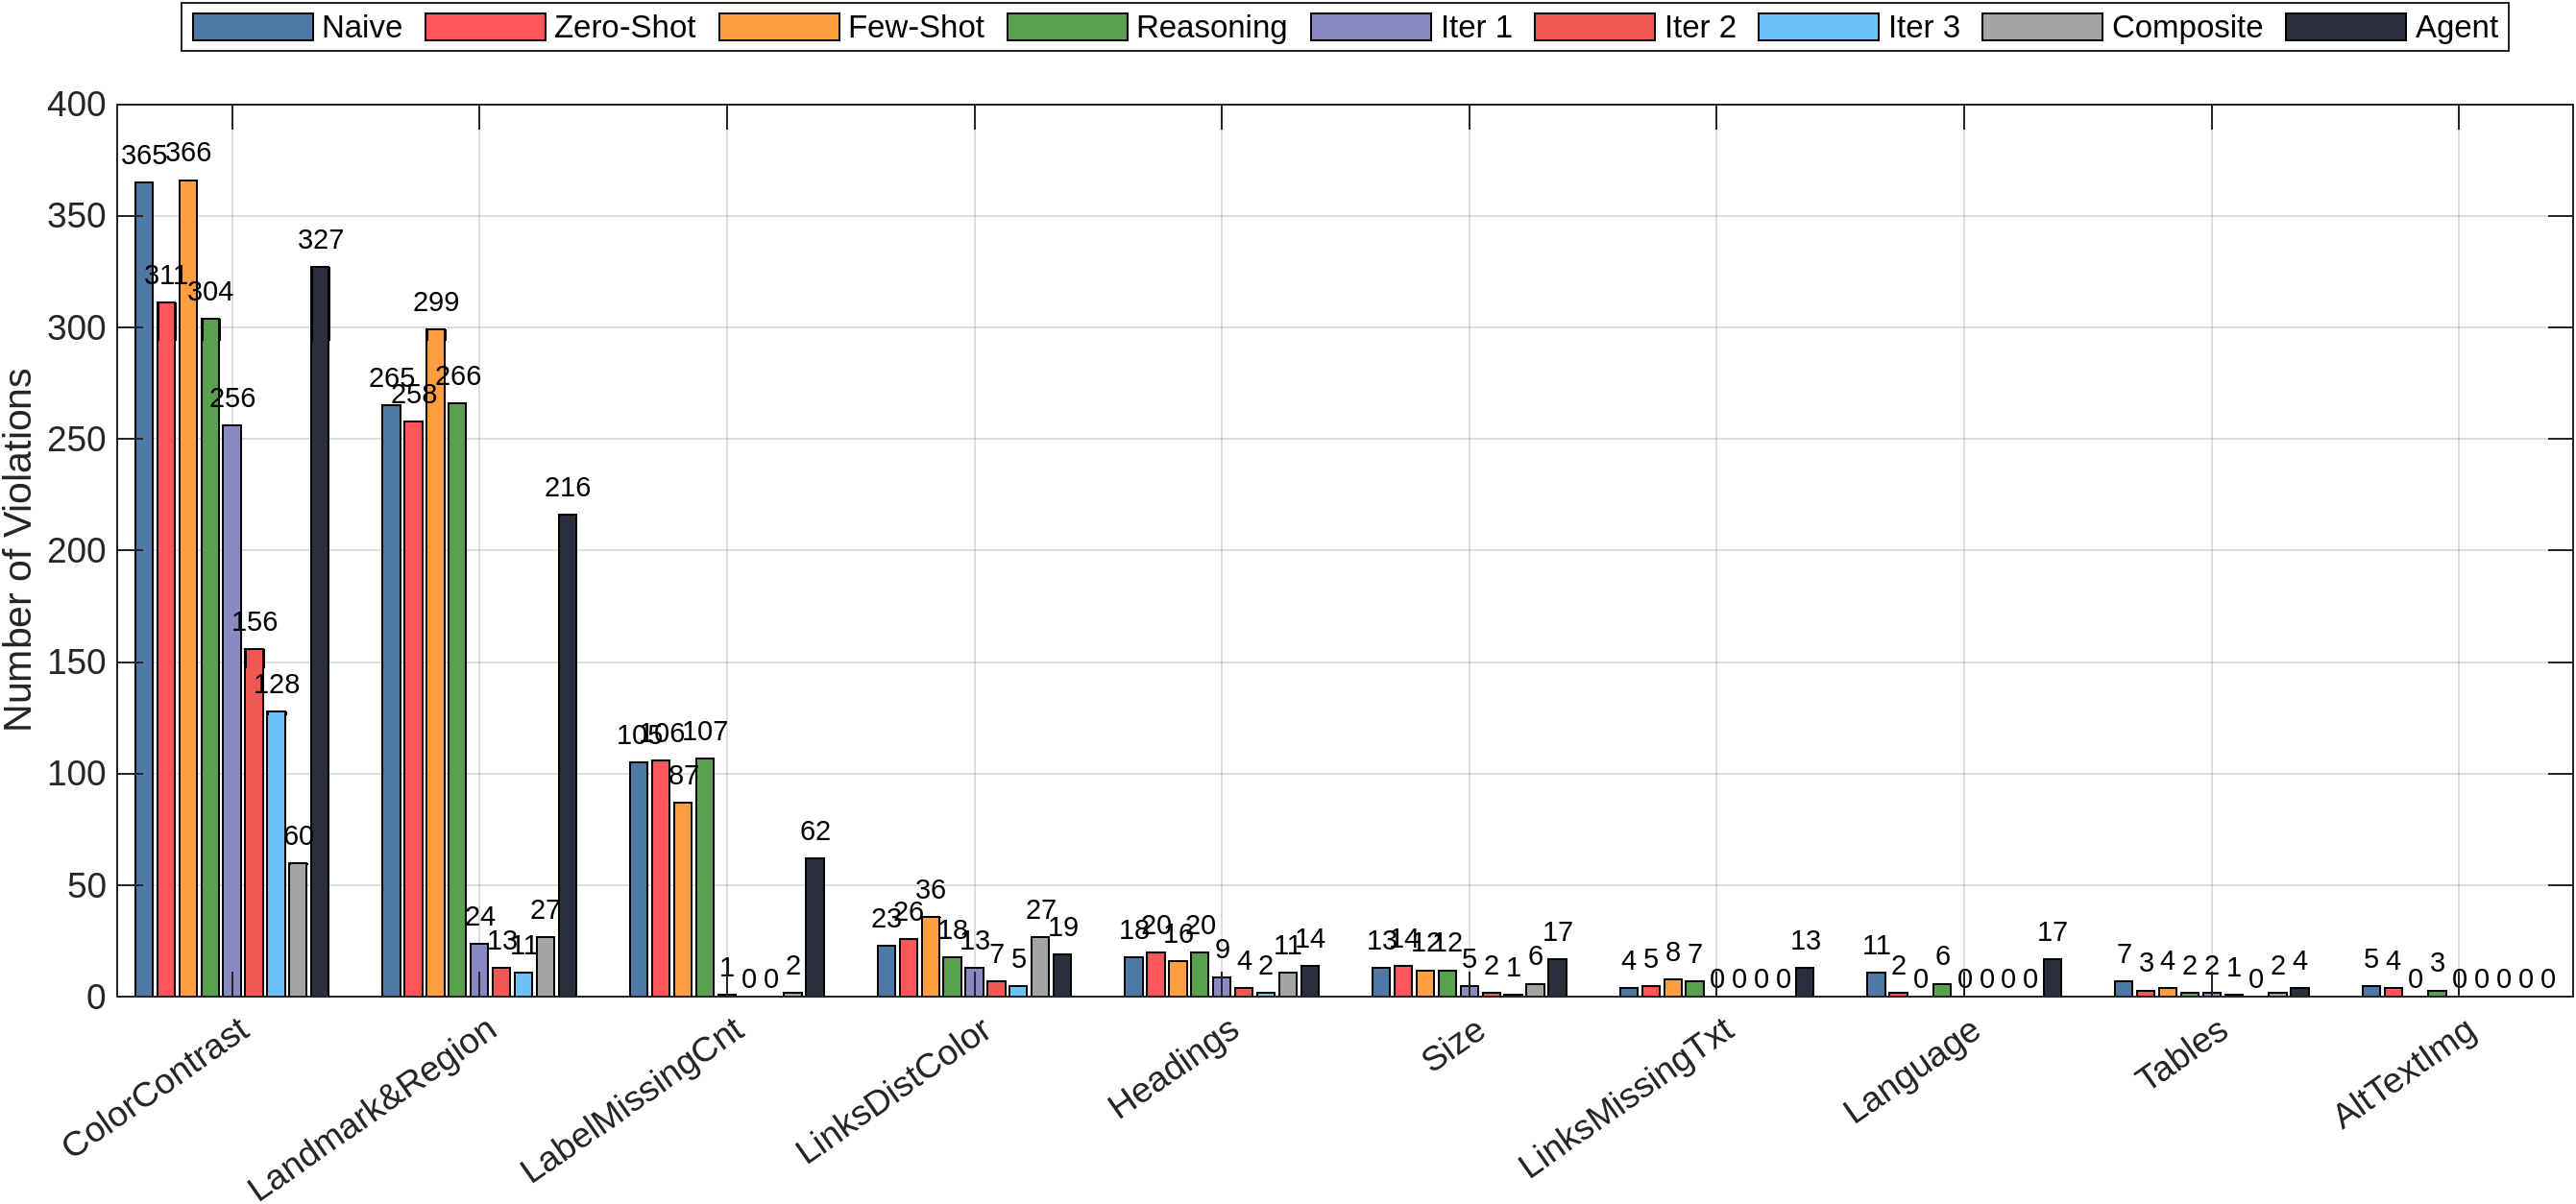
\includegraphics[width=\textwidth]{figures/gemini_wcag_bar.png}
%   \caption{Gemini: Distribution of WCAG violations across the dataset.}
%   \label{fig:gemini_wcag_bar}
% \end{figure*}


\subsubsection{Concentration of Violations}
While we do not know 
the exact training data of each model, we can infer by the observations that the 
models have been trained on similar underlying data. This also alligns with the 
error distribution of human developers, as WebAIM’s 2025 “Million” report shows.
In this report, 79\% (number check) of webpages fail the color contrast guidelines,
while 43\% (number check) of webpages do not use landmarks correctly. 
Combined with the other WCAG rules that can be found in non-negligible amounts, 
they are considered more complex and require a deeper understanding of the 
underlying HTML/CSS structure. \newline
This bias is faithfully reflected in the LLMs'
results, which gives us confidence to hypothesize that scraped code from 
forums like StackOverflow inforced this shortcut in the models' weights. 
Answers on forums often only start with the first <div> element, not showing 
the full page structure. This could explain the incorrect usage of landmarks and 
regions.

% \newcommand{\vect}[1]{\begin{pmatrix}#1\end{pmatrix}}
% \newcommand{\issues}{k}                   % Anzahl der Issue-Klassen
% \newcommand{\vx}{\mathbf x}
% \newcommand{\vy}{\mathbf y}

% \begin{enumerate}
%   \item \textbf{Amount of Issues}  
%         For each test run and file we are counting the number of violations per class
%         \[
%           \left(
%             \begin{array}{@{}l r@{}}
%               \text{Issue}_{1}: & x_{1}\\
%               \text{Issue}_{2}: & x_{2}\\
%               \vdots           & \vdots\\
%               \text{Issue}_{\issues}: & x_{\issues}
%             \end{array}
%           \right)
%           \xmapsto{\text{to vector}}
%           \vx \;:=\;
%           \vect{x_{1}\\x_{2}\\\vdots\\x_{\issues}} \in \mathbb R^{\issues}.
%         \]

%   \item \textbf{Calculation of Cosine Similarity}  
%         Given two experiment runs with $\vx,\vy\in\mathbb R^{\issues}$, we define
%         \[
%           \operatorname{cos\_sim}(\vx,\vy)=
%           \frac{\vx^{\mathsf T}\vy}{\lVert\vx\rVert\,\lVert\vy\rVert}
%           \quad\in[0,1].
%         \]
% \end{enumerate}

This cosine similarity is then plotted into a heatmap comparing the different 
experiment runs and files. The results can be seen in figure ab below. It 
is noticeable that most of the tiles show a bright color, referring to a 
high cosine similarity. The tiles with a darker color are mainly caused 
by 2 reasons. The first reason are files with only little violations 
that cause smaller cosine similarities due to the non-consistent 
distribution of violations. The second reason are randomly-generated 
files which have been mutated in such a way that they chose colors that 
comply with the Color Contrast Rules. Since overall the color constrast 
issues are one of the most common issues, this leads to a lower cosine 
similarity.\newline
Those findings are consistent different models and 
prompting techniques. This demonstrates that the accessibility issues are 
consistent across multiple runs and not caused by halluzination of the 
LLMs but are based on their training data and the underlying parameters.\newline
In a last step, the question arises why we see different results and 
violation distributions across the different models. Even though current 
LLMs are a \textit{black-box} regarding their training data and its impact, 
we can infer some possible bias based on recent accessibility studies. As 
the \textit{WebAIM 2025 Million} report~\parencite{webaim2025million} shows, 
79\% of all webpages contain low-contrast text. Similar results can be seen 
for WCAG landmark and region violations. 80,5\% of webpages contained at 
least one region, but only for 42,6\% a <main> element was present in the 
code. Other possible web-crawl training data sources like \textit{StackOverflow} 
and other forums could further bias the LLMs since they often start with 
the first <div> and omit the full page structure. This training data bias
could explain the observed differences in the amount and type of accessibility 
violations. Lastly, many of the observerd violations, such as color contrast
can be classified as more sophisticated, requiring a LLM to focus on the 
relative luminance and color contrast ratio. On the other hand, correct 
landmarks and regions require invisible semantics, apart from the raw pixel 
input of images. This semantic gap of information also requires deeper 
reasoning by the models. In conclusion, the observed violations follow 
a human bias which come from the vast training data that does not adhere 
fully to accessibility best practices.


\subsubsection{Dominance of Default Colors}
A further fine-grained analysis of the violations (Table xy) reveals that the 
majority of color contrast violations are caused by a small subset of colors.
After inspecting the most common colors, those colors can
be classified as \textit{default colors}. They are often used by browsers and 
popular frameworks and thus have been learned by the LLMs. For instance, we 
identified two public color palettes - the \textit{Google Color Palette} and the
\textit{Bootstrap v3-v5} - that explain a majority of the violation.
\begin{itemize}
  \item \textbf{Gemini.} 13 out of 127 colors that violate the color contrast 
  rules matches exactly one of the two color palettes. They are accounting for 
  65\% of all misses, 71\% if black (\#000000) and white (\#ffffff) are included.
  \item \textbf{GPT-4o.} 10 out of 237 colors match, leading to 24\% of all violations 
  (39\% if black and white are included).
\end{itemize}

Gemini appears to use a larger amount of boiler-plate colors, for instance 
using Bootstrap's link color \#007bff and its grey scale colors such as 
\#777777 - \#999999. \newline
On the other hand, apart from some default colors, GPT-4o uses a wider variety 
of colors. It appears that GPT-4o is more likely to mix its own colors into the
generated code, rather than relying on boiler-plate colors. This hypothesis
can be further supported by the fact that GPT-4o is able to solve a higher 
percentage of color contrast violations than Gemini. \newline


\begin{table}[ht]
\centering
\caption{Most common colors used by the LLMs.}
  \label{tab:colors}
  \begin{tabular}{lccc}
  \toprule
  Model        & Distinct Colors                 & Top-7 colors     & Percentage of       \\
               &         with Violations         &                  & all color contrast   \\ 
               &                                 &                  &  violations          \\ \midrule
  Gemini       & 127          & \#ffffff, \#777777, \#007bff, \#0000ee,  & 75\% \\
  Flash 2.0             &              & \#888888, \#999999, \#29abe2              &  \\
  GPT-4o       & 237          & \#ffffff, \#777777, \#888888, \#999999,  & 48\%  \\
      &              & \#ff0000, \#007bff, \#00ffff              &  \\
  Qwen 2.5-vl  & 0            &     & tbd \\
               &              &     &     \\
  \bottomrule
  \end{tabular}
\end{table}


\section{Image-to-Code Similarity}
\subsubsection{Prompting Techniques}
\subsubsection{Advanced Strategies}
Since Image-to-Code main task is to copy the input image as precise as possible,
we have analysed the performance across the different parameter sets to see how 
exact their results remain. The results in table as in the appendix 
indicate that the final scores decrease slightly when further accessibility 
instructions are mentioned to the LLMs. While the text and position similarity 
remains constant, the size and especially the text color similarity scores 
decrease. This is caused due to accessibility compliance that can cause the
LLMs to choose different colors and even component sizes to align with the 
WCAG issues. However, the changes in terms of the final score are very small 
and almost negligible.\newline
Overall, similar to former research gpt-4o demonstrates the best performance 
in this field by outperforming gemini flash-2.0 by a few percent.




